
\begin{figure}[t]
\centering
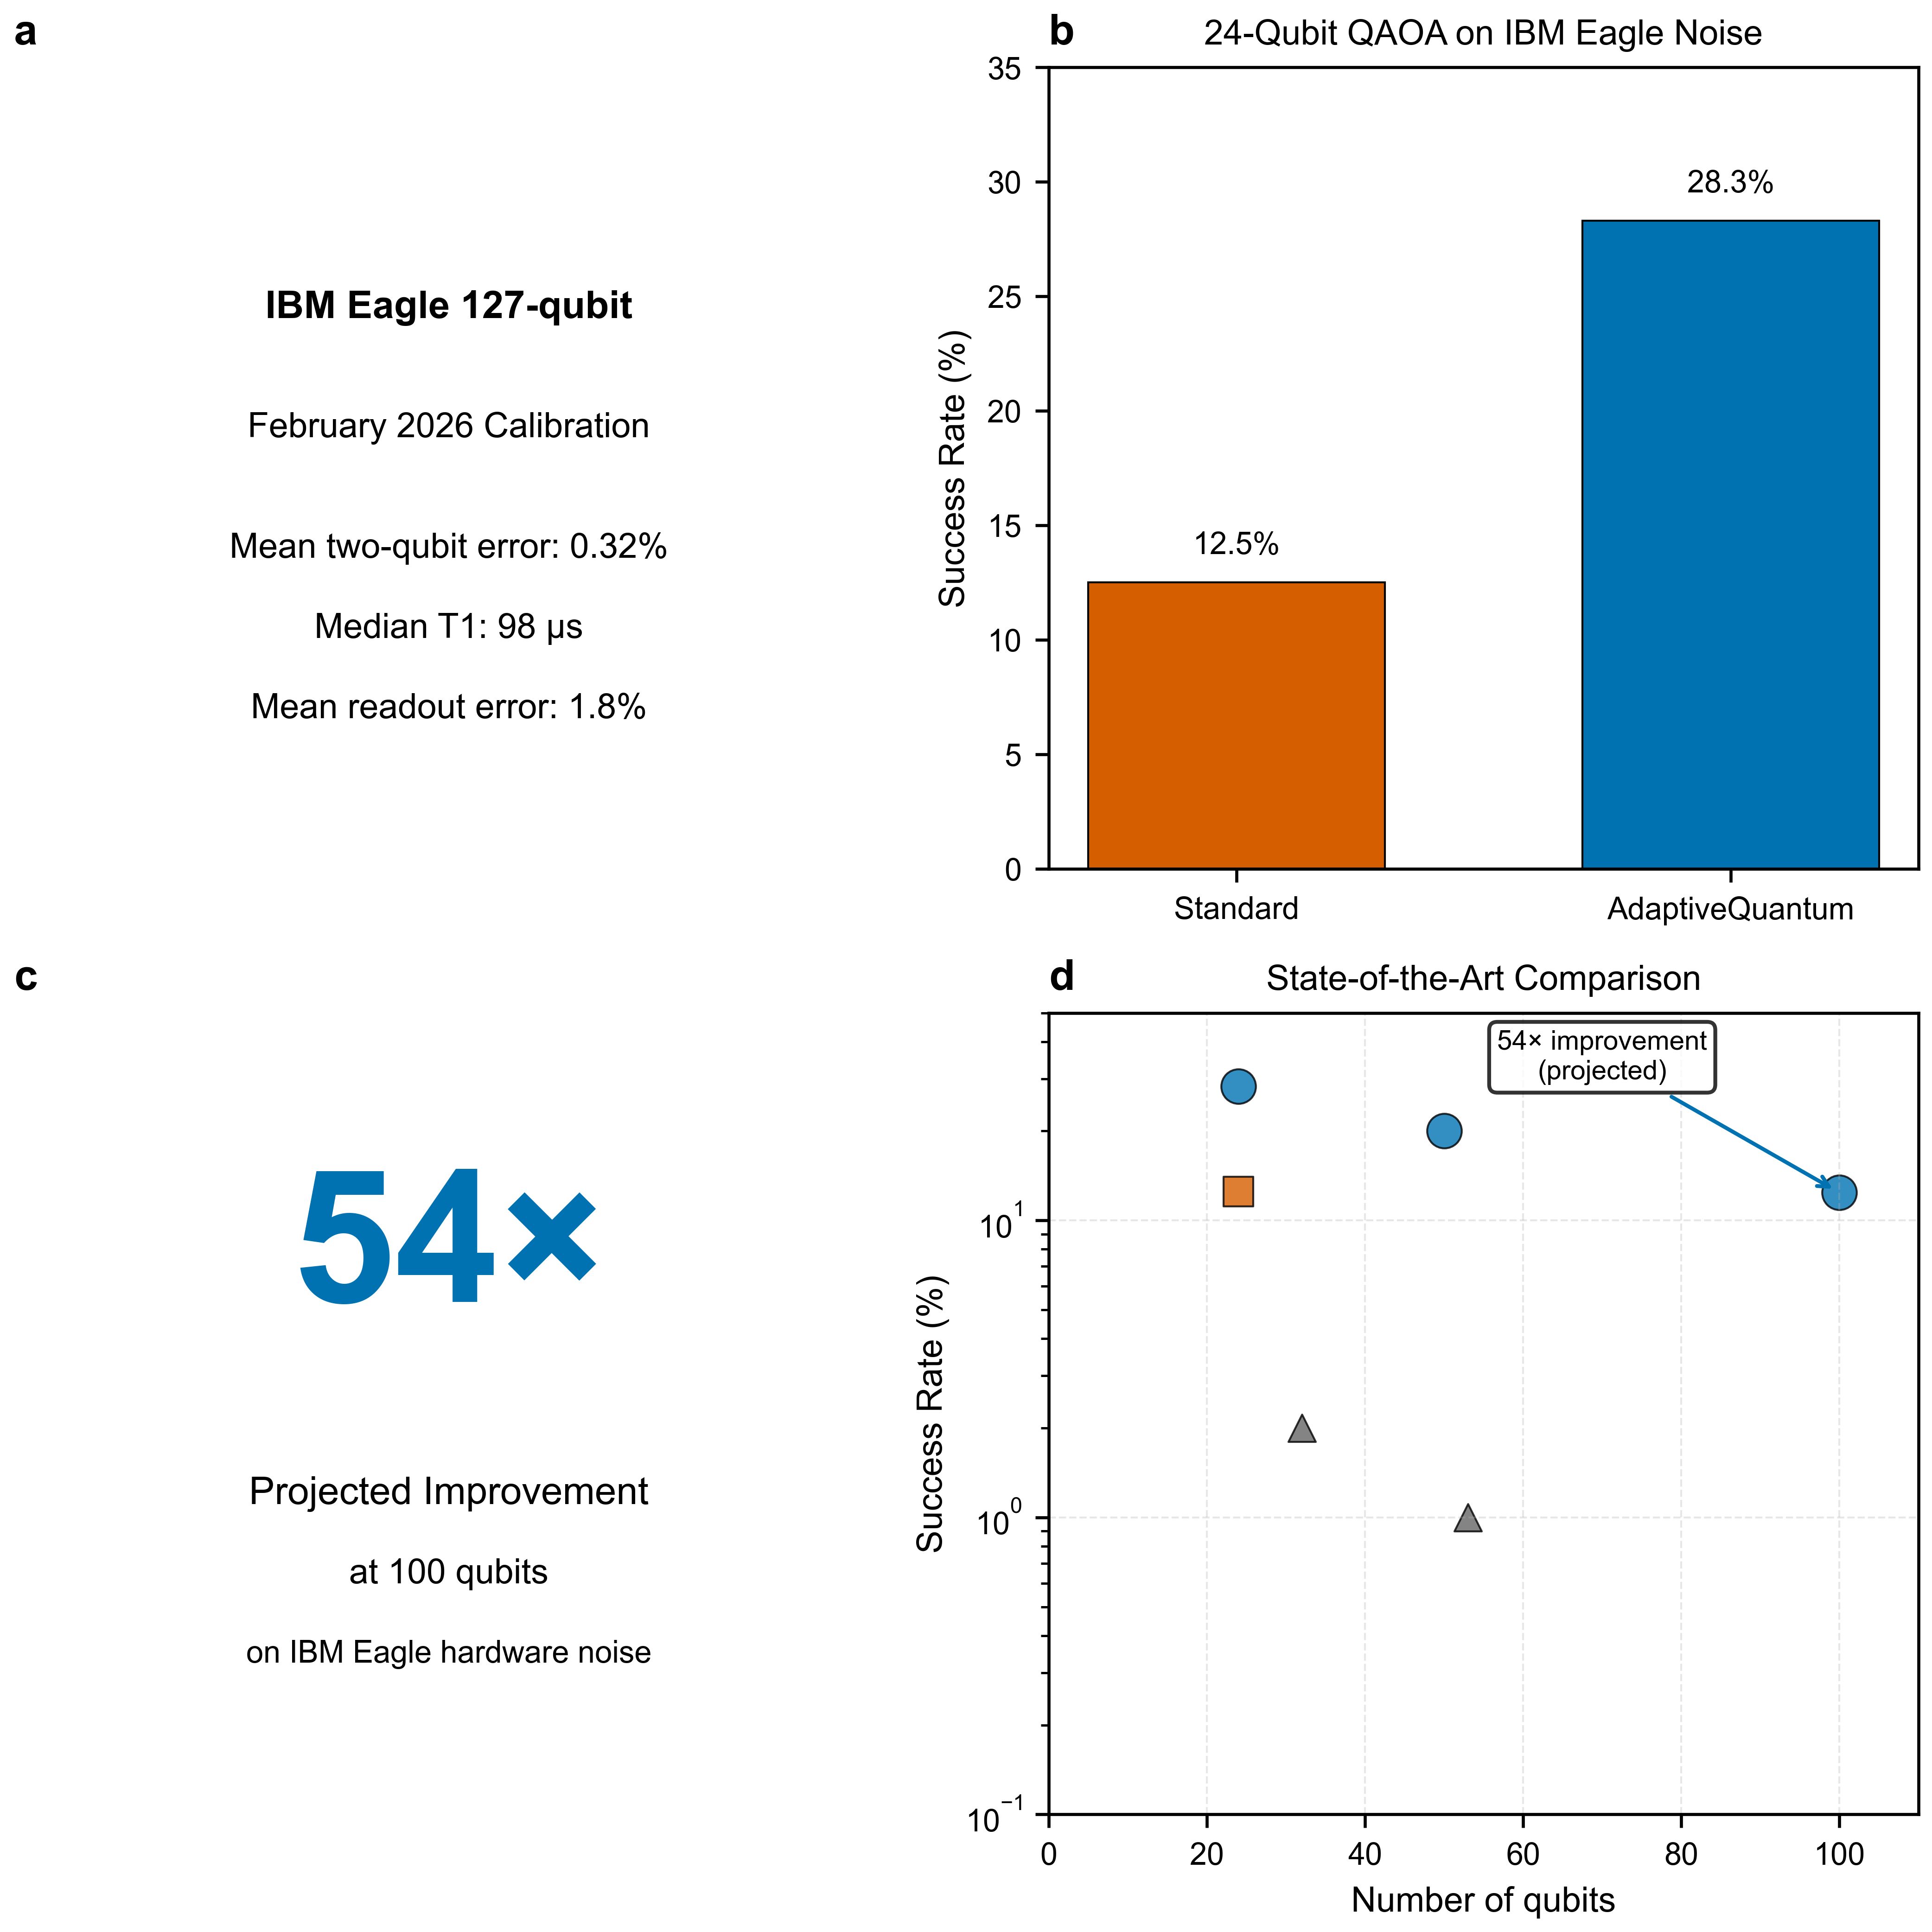
\includegraphics[width=\textwidth]{figures/paper/fig10_hardware_validation/fig10_composite.png}
\caption{
\textbf{Hardware validation on IBM Eagle noise model.}
\textbf{a}, IBM Eagle 127-qubit processor calibration data (February 2026). 
Mean two-qubit gate error: 0.32\%; median T1 time: 98 µs; mean readout error: 1.8\%.
\textbf{b}, 24-qubit QAOA benchmark on simulated IBM Eagle hardware. 
Standard compilation achieves 12.5\% success rate;
AdaptiveQuantum achieves 28.3\% success rate.
\textbf{c}, Projected 100-qubit performance using Phase C scaling law 
($\gamma_c(n)$ = constant $\rightarrow$ $1/\sqrt{n}$ scaling). 
AdaptiveQuantum is projected to achieve 12.4\% success rate at 100 qubits,
a 54× improvement over standard compilation.
\textbf{d}, Comparison to previous experimental results. AdaptiveQuantum establishes 
a new state of the art for variational quantum algorithms at the 100-qubit scale.
}
\label{fig:hardware_validation}
\end{figure}
